\documentclass[aspectratio=169]{beamer}
\usetheme{Boadilla}
\usepackage{tikz}
\usepackage{hyperref}
% \usepackage{enumitem}

\title{MTH 1030 Week 2 tutorial}
\author{Alex Elzenaar}


\begin{document}

\begin{frame}
  \begin{center}
    \textbf{MTH 1030---tutorial for week 2}\\
    Alex Elzenaar\\[1cm]
    \href{mailto:alexander.elzenaar@monash.edu}{alexander.elzenaar@monash.edu}
  \end{center}
  \begin{itemize}
    \item Email me about things like incorrectly entered grades.
    \item General course queries should go on the Moodle forum (you can also
    email me but my primary job is \textbf{not} teaching \& I will likely direct you to Moodle or the lecturers unless it is a very easy question).
    \item Requests to attend different tutorials should go to Eileen, her email is on Moodle. It is not in my power to deal with such things.
    \item Requests for compassionate consideration (eg assignment due date extensions) go via the university wide form linked on Moodle. Again I do not have authority to deal with queries about this.
  \end{itemize}
\end{frame}

\begin{frame}
  \begin{center}
    \textbf{What my research looks like}
  \end{center}
  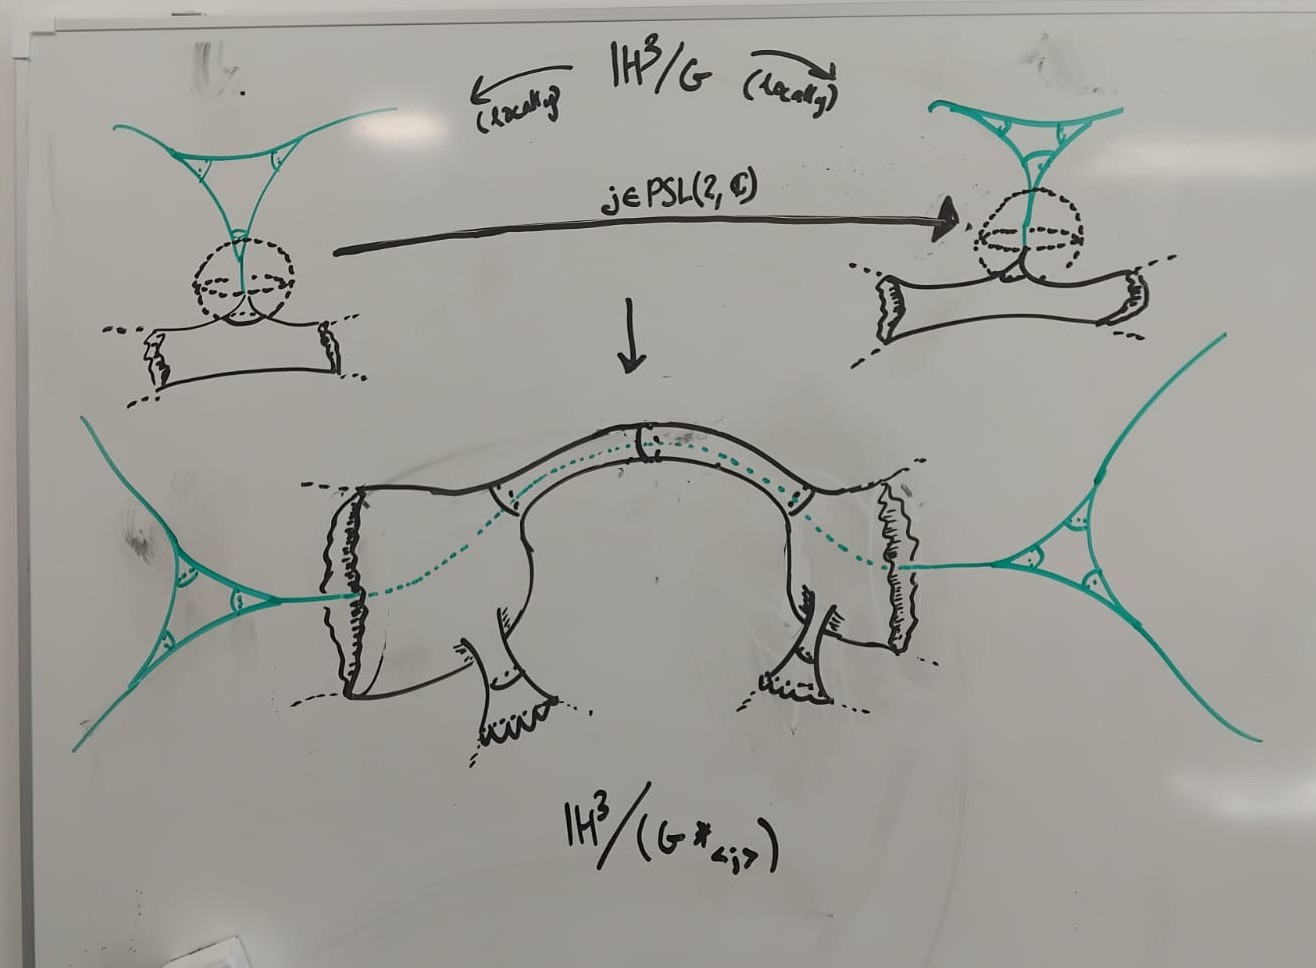
\includegraphics[height=.8\textheight]{../../cones/hnn_ext}
  \includegraphics[height=.8\textheight,page=7]{../../kg/talk2026_wurzburg.pdf}
\end{frame}

\begin{frame}
\begin{enumerate}
  \item Whiteboard markers, erasers, etc are in the box at the front. \textbf{If you find a marker that does not work, don't put it back in the box!!!}
  \item Get into groups of 3-4 people. Write your \textbf{preferred names} on the whiteboards so I can take attendance.
  \item Work on the questions \textbf{in your groups}. \textbf{Write your full thinking} on the boards, not just a final answer. You are
  graded in assignments/projects and the final exam on your reasoning and explanations, not just a final answer. If you don't practice in tutorials then I can't give any
  feedback before it starts to count for your grade.
  \item Try to keep screen use to a minimum. It's OK to look things up in the lecture notes but most of your time you should be at the whiteboard writing and talking to people.
        I am here to answer any questions about the content/questions, and I will be walking around, it is hard to help you if you are working on a screen and not the board.
  \item We will start to pack up for the quiz about 30min before the end.
\end{enumerate}
\end{frame}


\begin{frame}{Quiz}
\begin{enumerate}
  \item Please erase everything except your names so I can check attendance.
  \item You are not allowed to have anything open on your computer except the quiz. Including NO additional tabs open. Phones should be face down if they are not in your bag.
  \item When you have submitted the quiz put your hand up, when I have seen the submission screen I will check your attendance off. \textbf{If you leave without me seeing you
  have submitted the quiz you will not get an attendance grade.}
\end{enumerate}
\end{frame}

\end{document}
